%! Author = zhenxiang
%! Date = 23-3-23
% 关掉无意义的字体警告
\PassOptionsToPackage{quiet}{xeCJK}
\PassOptionsToPackage{quiet}{fontspec}
% Preamble
\documentclass[UTF8]{ctexart}

% Packages
\usepackage{amsmath}
% codes
\usepackage{listings}

% graphicx
\usepackage{graphicx}
% url
\usepackage{hyperref}
\hypersetup{
    colorlinks=true,
    linkcolor=blue,
    filecolor=magenta,      
    urlcolor=cyan,
    pdftitle={标题},
    pdfpagemode=FullScreen,
    }
% 页面设置
\usepackage{geometry}
\geometry{left=2.5cm, right=2.5cm, top=2.5cm, bottom=2.5cm}
% Document
\begin{document}

\section{环境配置}

参考这个网站的
\href{http://doraemonzzz.com/2022/12/25/2022-12-25-ECE408-\%E7\%8E\%AF\%E5\%A2\%83\%E9\%85\%8D\%E7\%BD\%AE\%E4\%BB\%A5\%E5\%8F\%8ALab-0/#Lab-0}{环境配置}\\



\begin{lstlisting}[language=bash]
git clone https://github.com/abduld/libwb.git
cd libwb
make all

# 添加环境变量,将上面的libwb目录添加到.bashrc(.zshrc)文件中
export WB_DIR=path_2_libwb

# 在MP0中添加makefile
WB = ${WB_DIR}

template.o: template.cu
	nvcc -std=c++11 -rdc=true -I $(WB) -c template.cu -o template.o

solution: template.o
	nvcc -std=c++11 -o solution template.o $(WB)/lib/libwb.so

clean:
	-rm -f template.o
	-rm -f solution

# 在上面makefile目录下执行
make solution
./solution
\end{lstlisting}

\newpage
实验结果如下(截图)
% 图片置于当前位置
\begin{figure}[ht]
    \centering
    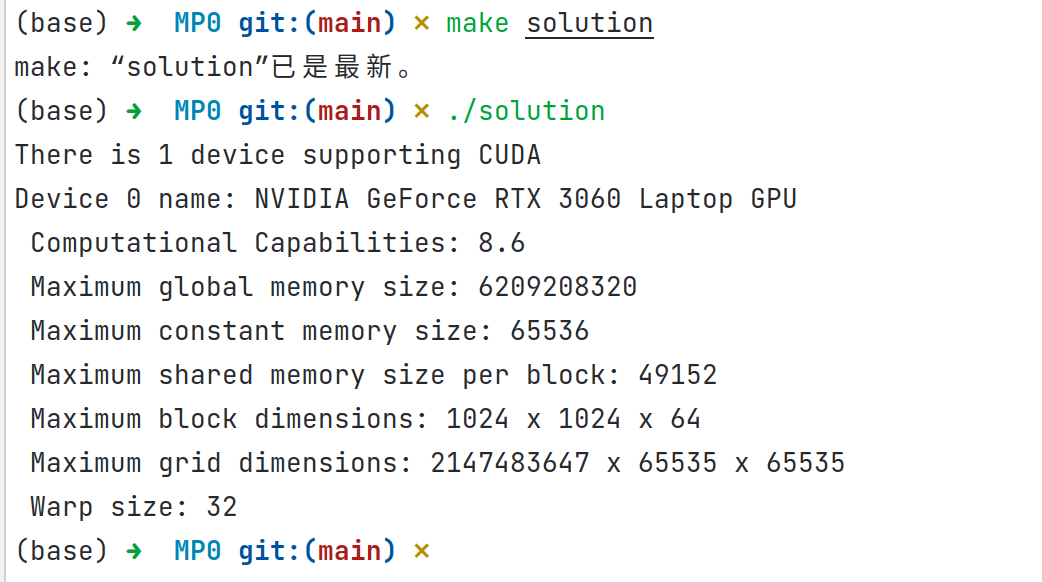
\includegraphics[width=1.0\textwidth]{photos/lab0.png}
    \caption{lab0实验结果}
    \label{fig:1}
\end{figure}



\end{document}